\documentclass[a4paper]{article}

\usepackage{amsmath} 
\usepackage{amsfonts}
\usepackage[shortlabels]{enumitem}
\usepackage{array}
\usepackage{graphicx}
\usepackage{pgfplotstable}
\begin{document}  
\title{Mathematics Examination}
\date{DD-MM-YYYY}
\author{Rujuta Budke}
\maketitle

\newpage
\tableofcontents
\newpage

\begin{Large}
\underline{Instructions:}\\
\end{Large}


\noindent \textbf{Duration: 2hrs} \hfill \textbf{Time: 2hrs}
\begin{enumerate}
\item Write your MIS number on paper 
\item Unless otherwise mentioned symbols and notations have their usual standard meaning
\item Use of any kind of electronic device is NOT allowed
\item Any essential result, formula or theorem assumed for answering of questions must be clearly stated.
\end{enumerate}



\pagebreak

\section{Logical Reasoning}

\subsection*{Question I}
1. Establish the logical equivalence, where \textit{x} does not occur as a free variable in A. Assume that domain is non-empty. \hfill [CO3][{\bf 1}]
\begin{center}
$ \forall x (A \implies P(x))\equiv \forall x (A \lor P(x))$
\end{center}

2. Find the conjunction of the propositions \textit{p} and \textit{q} where \textit{p} is the proposition "Rebecca's PC has more than 16GB free hard disk space" and \textit{q} is the proposition "The processor in Rebecca's PC runs faster than 1 GHz'"\hfill [CO1][{\bf 1}]

\subsection*{Question II}
1. Let \textit{p} and \textit{q} be the propositions "The election is decided" and "The votes have been counted," respectively. Express each of the following compound propositions as an English sentence. \hfill [CO2][{\bf 2}]
\begin{enumerate}[a)]
\item $\neg p \land q$
\item $ p \iff q $
\end{enumerate} 
2. Determine the truth value of the each of these domains if the domain consists of all real numbers.\hfill [CO2][{\bf 2}]
\begin{enumerate}[a)]
\item $\exists x (x^3 = -1) $
\item $\forall x((-x)^2 = x^2)$
\end{enumerate} 


\newpage
\section{Algebra}
\subsection*{Question I}
1. Find eigenvalues and corresponding eigenvectors of A = 
	$\begin{bmatrix}
	2 & -1 \\ -1 & 2
	\end{bmatrix}$. Hence, find an orthogonal basis for $ \mathbb{R}  ^2$ \cite{real}
	\hfill [CO2][{\bf 2}]\\ \\
2. Find the rank of matrix $
	\begin{bmatrix}
	8 & 6 & 4 & 1 & 3\\
	2 & 1 & -7 & 4 & 1\\	
	1 & 1 & -1 & 2 & 1\\
	1 & -1 & 2 & 0 & 0\\
	\end{bmatrix}$ 
	\hfill [CO3][{\bf 3}]
\subsection*{Question II}
1. Determine whether $\lbrace 1, x^2, x^2 + 2 \rbrace$ spans $P_2(\mathbb{R})$. Is it linearly independent? Justify your answers.\hfill [CO4][{\bf 1}]\\ \\
2. Let V be a vector space. Prove that $W_1$ and $W_2$  are subspaces of V then their intersection $W_1 \cup W_2$ is a subspace of V.\hfill [CO2][{\bf 2}]
\newpage
\section{Calculus}
\subsection*{Question I}
%nested lists
\begin{enumerate}
\item Attempt the following questions:
	\begin{enumerate}[a)]
	\item Find the particular solution of the initial value problem: \hfill [CO2][{\bf 2}]
	
		\begin{align*}
	\tan x\frac{dy}{dx}&=y
	\\y(\frac{\pi}{2})&=(\frac{\pi}{2})
		\end{align*} 
	
	\item Check the whether the following differential equation is exact or non-exact and justify your answer.\hfill [CO2][{\bf 2}]
	 	\begin{equation*}
	 (1 + \ln xy)dx + (1 + \frac{x}{y})dy = 0
		\end{equation*} 
	\end{enumerate}
\item Find a second order homogeneous LDE for which following are LI solutions: $ e^{-kx}\cos {\pi x}, e^{-kx}\sin {\pi x} $ \hfill [CO3][{\bf 2}]
\end{enumerate}

\subsection*{Question II}
\begin{enumerate}
\item Solve using variation of parameters\hfill [CO3][{\bf 4}]
	\begin{enumerate}[i)]
	\item $ y'' + 4y = \cos{2x} $
	\item $(D^2 + 2D + 2I)y = 4e^{-x} \sec^3 x $
	\end{enumerate}
\item Solve the following non-homogeneous LDE using the method of undetermined coefficients:\hfill [CO5][{\bf 4}]
	\begin{enumerate}[i)]
	\item $y'' - 4y' = 8 \cos {\pi x}$
	\item $(D^2 - I)y = \sinh x $
	\end{enumerate}
\item Solve: $ \int \frac{x}{x(x+1)(x+2)} \ dx $\hfill [CO3][{\bf 2}]
\end{enumerate}


\newpage
\section{Image-based}
\subsection*{Question I}
If 1 litre of water (about 1.06 US quart) is vibrating up and down under the influence of gravitational in a U-shaped tube of diameter 3cm (Fig 1.), what is the frequency? Neglect friction.\cite{img}

\begin{figure}[h] 
\begin{center}
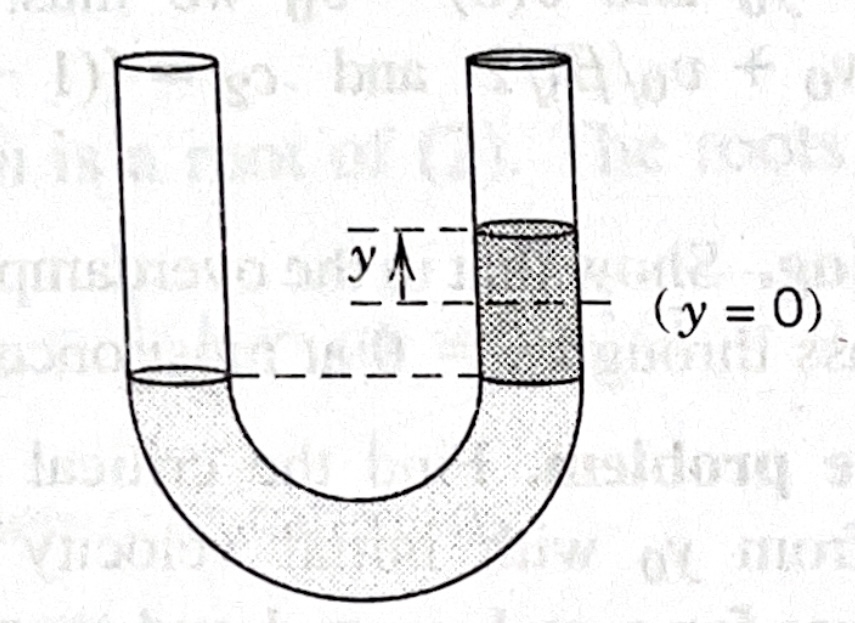
\includegraphics[width=.25\textwidth]{tube}
\caption{Tube (Question 1)}
 \label{fig1}
\end{center}
\end{figure}

\subsection*{Question II}
What are the frequencies of vibration of bpdy of mass m = 5kg i) on a spring of modulus $k_1 = 20 nt/m$, ii) on a spring of modulus $k_2 = 45 nt/m$, iii) on the two spring in parallel? See Fig. 2.
\cite{img}
\begin{figure}[h] 
 \begin{center}
  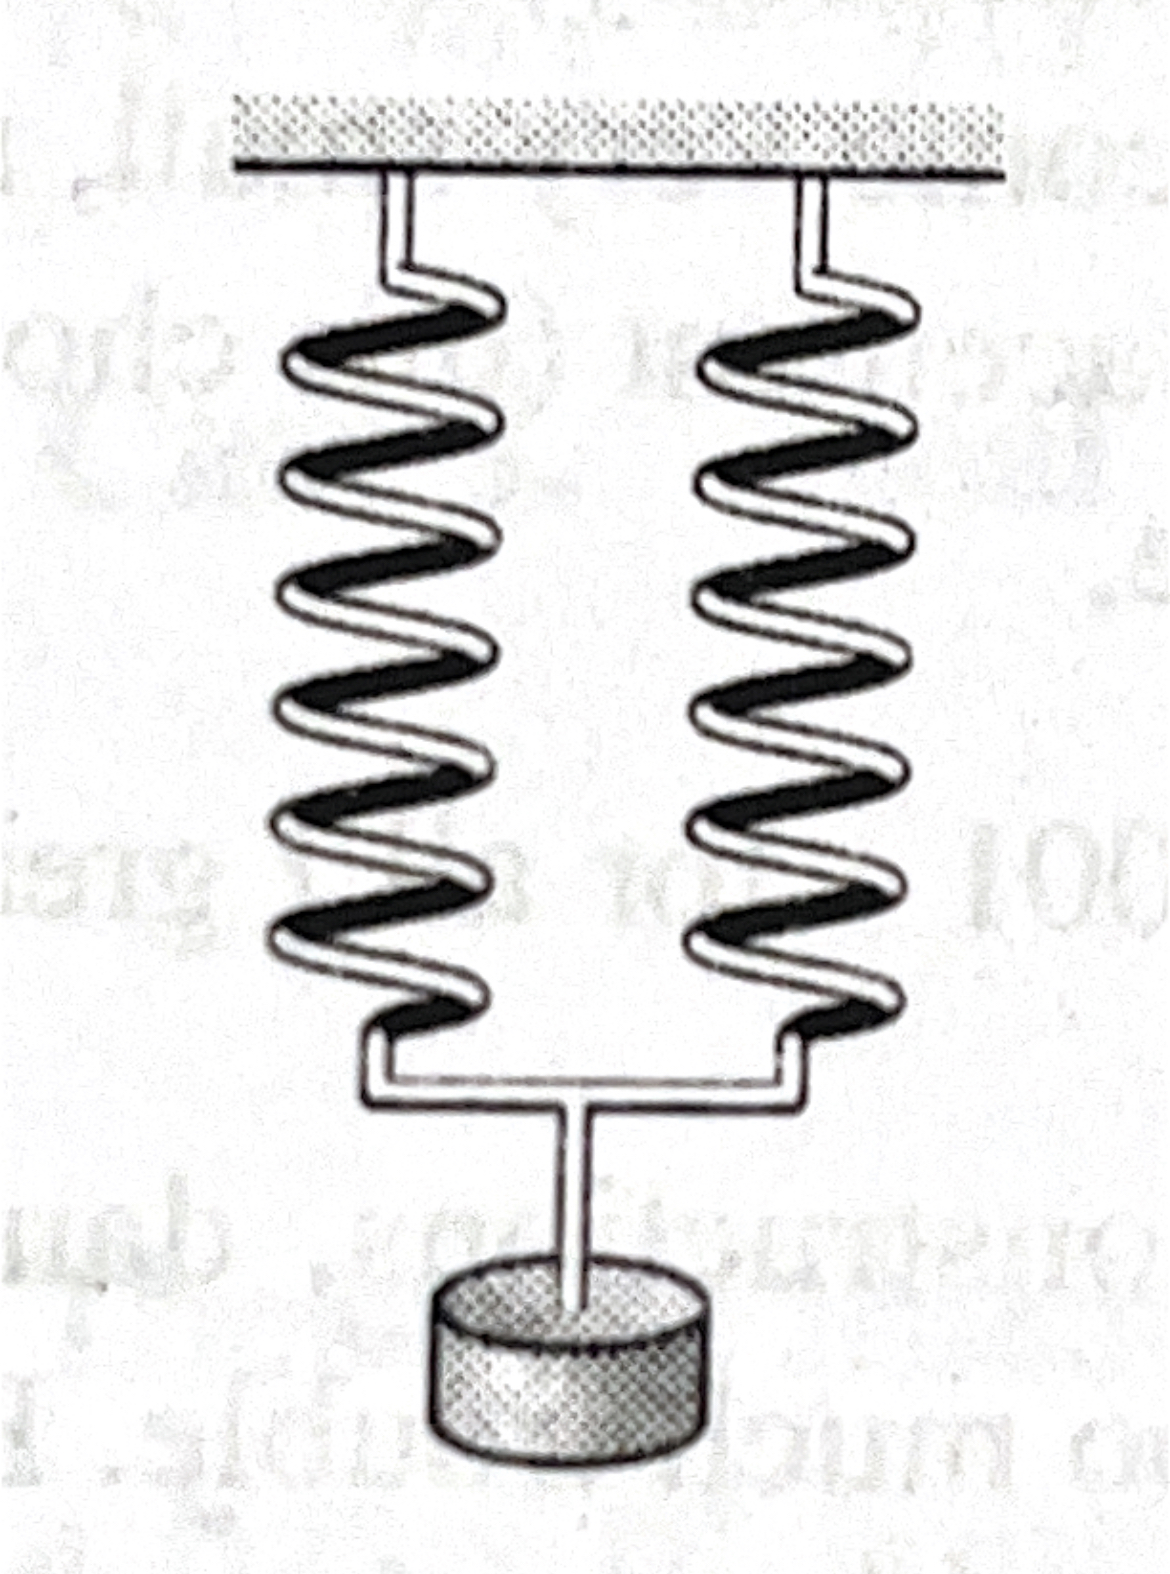
\includegraphics[width=.25\textwidth]{spring}
  \caption{Spring (question 2)}
 \label{fig2}
 \end{center}
\end{figure} 


\newpage
\section{Tables}
\subsection*{Question I}
Study the following table and answer the questions based on it. \cite{float}

\begin{table}[h] 
\begin{tabular}{|l|c|c|c|c|r|}
\hline
Year & \multicolumn{4}{c}{Item of Expenditure} \\
& Salary & Fuel and Transport & Bonus & Interest of Loans & Taxes\\
 \hline
 1998 & 288 & 98 & 3.00 & 23.4 & 83 \\ 
  \hline
 1999 & 342 & 112 & 2.52 & 32.5 & 108 \\ 
  \hline
 2000 & 324 & 101 & 3.84 & 41.6 & 74 \\ 
 \hline
 2001 & 336 & 133 & 3.68 & 36.4 & 88 \\ 
 \hline
 2002 & 420 & 142 & 3.96 & 49.4 & 98 \\ 
 \hline
\end{tabular}
\caption{\label{Question I} Expenditures of a Company (in Lakh Rupees) per Annum Over the given Years.}
\end{table}


\begin{enumerate}
\item What is the average amount of interest per year which the company had to pay during this period?
\item The total amount of bonus paid by the company during the given period is approximately what percent of the total amount of salary paid during this period?
\item Total expenditure on all these items in 1998 was approximately what percent of the total expenditure in 2002?
\item The total expenditure of the company over these items during the year 2000 is?
\item The ratio between the total expenditure on Taxes for all the years and the total expenditure on Fuel and Transport for all the years respectively is approximately?
\end{enumerate}

\subsection*{Question II}

\begin{table}[h]
\begin{tabular}{|l|c|c|c|c|c|r|}
\hline
	& \multicolumn{6}{c}{Subject (Max. Marks)} \\
 Student & Maths	 & Chemistry	 & Physics & Geography & History & Computer Science \\

& (150) & (130) & (120) & (100) & (60) & (40) \\
\hline
Ayush	& 90 &	50	& 90	 & 60 & 70  &	80 \\
Aman	 & 100	& 80	 & 80	& 40	 & 80 &	70 \\
Sajal	& 90 &	60 & 	70 & 	70	& 90	 & 70 \\
Rohit	& 80 & 	65 & 	80	& 80	 & 60 &	60 \\
Muskan	& 80 &	65	& 85	 & 95	& 50	 & 90 \\
Tanvi	& 70	 & 75	& 65	 & 85	& 40 &	60 \\
Tarun	& 65 &	35	& 50	 & 77	& 80	 & 80 \\
\hline
\end{tabular}
\end{table}
\noindent \cite{float} The above table gives the percentage of marks obtained by seven students in six different subjects in an examination. \\ 
\textit{The numbers in the brackets give the maximum marks in each subject.}

\begin{enumerate}
\item What are the average marks obtained by all the seven students in Physics? (rounded off to two digit after decimal)
\item The number of students who obtained 60% and above marks in all subjects is?
\item What was the aggregate of marks obtained by Sajal in all the six subjects?
\item In which subject is the overall percentage the best?
\item What is the overall percentage of Tarun?
\end{enumerate}
\pagebreak
\section{Tables using CSV}
\subsection*{Question I}
\begin{table}[h]
  \begin{center}
    \caption{Autogenerated table from .csv file.}
    \label{table1}
    \pgfplotstabletypeset[
	col sep=comma,
	columns/Year/.style={string type},
	every head row/.style={before row=\hline,after row=\hline},	% style the first row
	every last row/.style={after row=\hline},	% style the last row
	every first column/.style={column type/.add={|}{}},	% style the first column
	every last column/.style={column type/.add={}{|}},
]{data.csv} % filename/path to file
  \end{center}
\end{table}
\begin{enumerate}
\item For which set of years of the combined consumption per day is equal with other set of years?
\item What is the percentage of average consumption of wheat for the given set of years to average consumption of total grains?(approx)
\item For which food grain consumption, was there successive increase over the given set of years?
\end{enumerate}
\pagebreak
\begin{thebibliography} {}
\bibitem {float} Float, LaTeX Stack Exchange, $tex.stackexchange.com/questions/2275/keeping-tables-figures-close-to-where-they-are-mentioned$ 
\bibitem{real} Real Number Symbol in LaTeX, $https://www.physicsread.com/latex-real-number/$
\bibitem {img}Adding Images, Overleaf, $www.overleaf.com/learn/latex/Inserting_Images$
\bibitem {bib}Bibliography management with bibtex, Overleaf, $www.overleaf.com/learn/latex/Bibliography_management_with_bibtex$

\end{thebibliography} 
\end{document}  

